\documentclass{article}
\usepackage{longtable}
\usepackage{geometry}
\usepackage{hyperref}
\usepackage{graphicx}
\usepackage{float}
\usepackage{cite}
\linespread{1.2}

\begin{document}
\begin{titlepage}
    \centering
    % Add your title, author, date, and other information here
    
\includegraphics[scale = 0.6]{logo.jpg}
    \\---------------------------------------------------------------------------------------------------------------------------------
    \vspace{0.5cm}
    \\\huge\textbf{Waste Classification through Image Processing}\par
    \vspace{0.5cm}
    \Large{CS 446: App. Digital Image Processing}\par
    \vspace{1.5cm}
    \large\textbf{Members:}
    \\ \large{Zainab Haider - 07104}
    \\ \large{Bushraa Yousuf - 07609}
    \vspace{0.5cm}
    \\\large\textbf{Instructor:}
    \\\large{Dr. M. Mobeen Movania}
    \vspace{0.5cm}
    \\\large\textbf{Section:}
    \\\large{L1}
    \vspace{1.7cm}
    \\\large{From the department of Computer Science}
    \\\large{Dhanani School of Science and Engineering}
    \\\large{Habib University}
    \\\large{\today}
\end{titlepage}

\tableofcontents
\vspace{7.3cm}
\section{Introduction}

\section{Motivation}

\section{Novel Idea}

\section{Mathematical Model}
For image classification, we will be using CNN(Convolutional Neural Network). CNN is made up of different layers. Below is the standard mathematical model for the different layers of CNN:
\begin{enumerate}
    \item \textbf{Convolutional layer}
    \\ 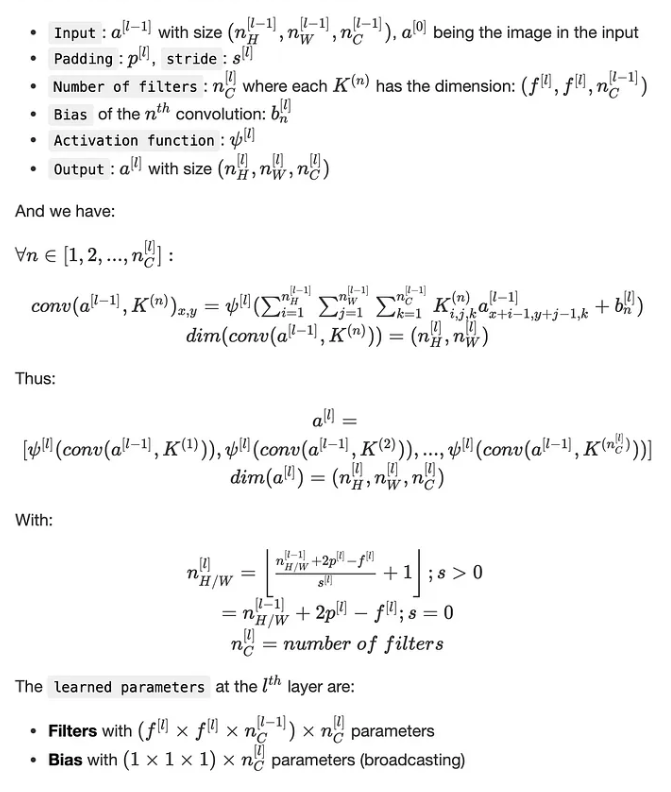
\includegraphics[scale = 0.6]{1st.png}
    \item \textbf{Pooling layer}
    \\ 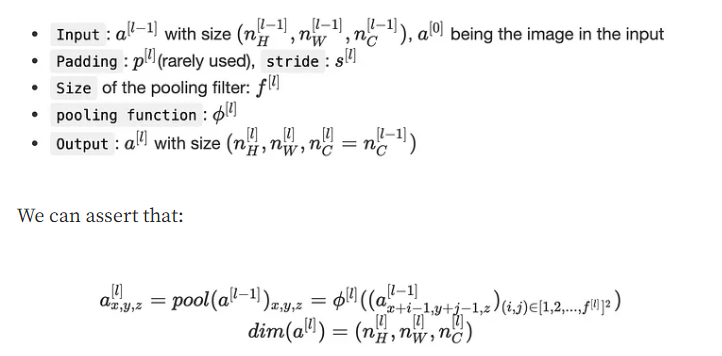
\includegraphics[scale = 0.69]{2nd.png}
    \item \textbf{Fully connected layer}
    \\ 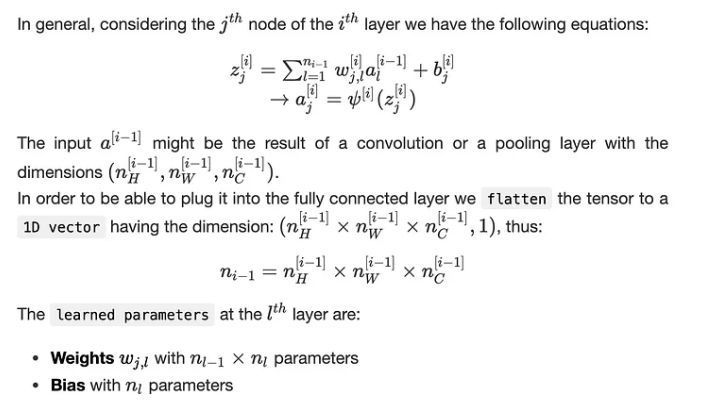
\includegraphics[scale = 0.69]{3rd.png}
\end{enumerate}
The following illustruation can sum up the the working of these layers:
\\ 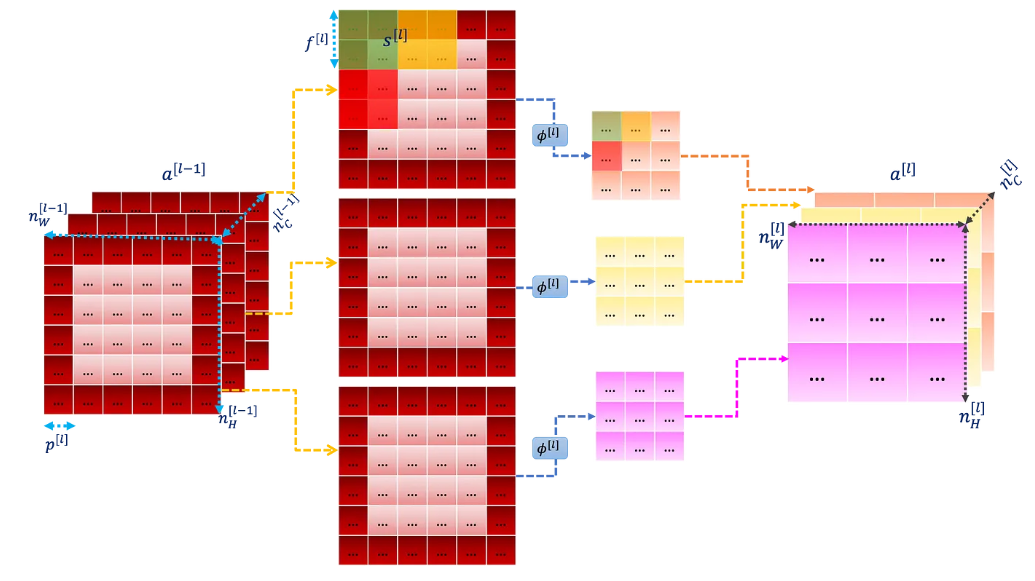
\includegraphics[scale = 0.55]{4th.png}    
\section{Relevance in Local Context}

Pakistan grapples with a significant solid waste management challenge, producing a staggering 49.6 million tons of waste annually, a number increasing at a rate of over 2.4 percent each year. Unfortunately, only a meager 13 to 23 percent of this waste is recycled due to the absence of a well-established recycling industry and the predominant reliance on manual sorting methods.

In this landscape, the development of a project like ours, focusing on efficient garbage classification, stands as a pivotal step towards addressing these issues. Introducing advanced waste sorting technologies and processes serves as a stepping stone in the foundation for a much-needed recycling industry in Pakistan. Such an industry holds multifaceted benefits for the nation.

Furthermore, a thriving recycling industry can play a pivotal role in reducing environmental pollution. By diverting a significant portion of waste from landfills and incineration, it minimizes harmful emissions and prevents soil and water contamination. This translates into cleaner air, water, and land for urban and rural areas. Additionally, recycling conserves valuable natural resources, reducing the need for the extraction and processing of new raw materials. This not only eases the strain on ecosystems but also lowers energy consumption, contributing to a more sustainable and eco-friendly future for Pakistan.
\section{Project Plan}
The table below gives the tentative project plan we will be following:
\begin{center}
\begin{table}[H]
\centering
\begin{longtable}{|c|p{0.6\textwidth}|c|}
\hline
Phase & Description & Duration \\
\hline
Literature Review & Our research initiative involves a comprehensive review of existing work on our chosen topic, comparing various approaches. A key focus is studying Convolutional Neural Networks (CNNs) for image classification, dissecting their architectures and performance metrics. Through this analysis, we aim to find new ways to contribute to this field, ultimately finalizing our project plan. & 2 weeks \\
\endfirsthead
\hline
Image Processing and implementation & Our next phase of the project involves delving into the image processing component. We will begin by gathering the necessary data for our research, followed by the implementation and training of our Convolutional Neural Network (CNN) model. Rigorous testing will ensue to evaluate its performance. Concurrently, we'll actively seek opportunities to refine and enhance the model's functionality, ensuring it aligns seamlessly with our project goals. & 6-8 weeks \\
\hline
GUI interface implementation & In the project's final stage, we'll develop a user-friendly GUI, emphasizing a sleek appearance and ease of use. This essential step will ensure a polished and inviting interface, aligning our project with user expectations and marking its completion. & 2 weeks \\\hline
\end{longtable}
\end{table}
\end{center}

\section{Team Distribution}
As there are only two individuals in our group, we will collaborate closely on most tasks, and the workload will be shared evenly between us. The table below gives deatils on the work distribution:\\ \\ 
    \centering
    \begin{tabular}{|c|c|}
        \hline
        Member & Distribution         \\ \hline
        Zainab Haider    & 50\%   \\ \hline
        Bushraa Yousuf    & 50\%  \\ \hline
    \end{tabular}
\begin{thebibliography}{9}
  \bibitem{GeeksForGeeks}
  International Trade Administration. \textit{} [Online]. Available: https://www.trade.gov/country-commercial-guides/pakistan-waste-management
  
  \bibitem{Brilliant}
  Dawn News. \textit{} [Online]. Available: https://www.dawn.com/news/1505436.
  \bibitem{Brilliant}
  Arab News. \textit{} [Online]. Available: https://www.arabnews.pk/node/1894661.
  \bibitem{Brilliant}
  Medium. \textit{} [Online]. Available: https://towardsdatascience.com/convolutional-neural-networks-mathematics-1beb3e6447c0.
 
    \end{thebibliography}
\end{document}
